\chapter{PLANO DE TRABALHO}
\label{chap:planoTrabalho}

\section{TECNOLOGIAS E FERRAMENTAS}
\label{sec:tecnologiasFerramentas}
Para a implementação do \textit{front-end} do sistema web foi utilizado o framework javascript \textit{React.js}, devido a sua capacidade de construção de \textit{Single Page Applications} (SPAs), que permitem a interação do usuário com as páginas da aplicação sem demandar de recarregamento das páginas.
Nas \textit{SPAs} todo os \textit{templates}, ou seja, códigos \textit{HTML}, \textit{CSS} e \textit{Javascript} dos quais o navegador necessita interpretar para a renderização das páginas, são carregadas no inicio do uso da aplicação, restando somente o carregamento dos dados a serem feitos com as mudanças de telas.

\citeonline{Tesarik2008} mostram em seu trabalho as dificuldades na construção de SPAs por conta do design mais sofisticado que esta deve ter para permitir a movimentação do usuário entre as páginas. 
Mas em contrapartida apresentam uma das principais vantagens deste tipo de construção, que é a melhor fluidez que pode ser obtida na experiência do usuário ao interagir com a aplicação.

Em conjunto ao React.js foram utilizadas as seguintes bibliotecas: 

\begin{itemize}[topsep=5pt]
    \item \textbf{Bootstrap\footnote{Disponível em https://getbootstrap.com/}:} É um pacote de ferramentas para construção do lado do cliente da aplicação, ou seja, o \textit{front-end}. Contém componentes que facilitam a construção e estilização de páginas responsivas, disponibilizando recursos em \textit{HTML}, \textit{CSS} e \textit{Javascript}.  
    \item \textbf{Charts.js\footnote{Disponível em https://chartjs.org/}:} É uma biblioteca rápida, responsiva e flexível utilizada por designers e desenvolvedores para a construção de gráficos.
    \item \textbf{D3.js\footnote{Disponível em https://d3js.org }:} Abreviação para \textit{Data-Driven Documents}, ela é uma biblioteca para criação dinâmica e interativa de gráficos, grafos e outras ferramentas de visualização de dados.
\end{itemize}

Para a implementação do \textit{back-end} foram criados dois programas isolados. 
O primeiro consiste de uma \textit{API} construída utilizando a plataforma Node.js com a linguagem de programação \textit{Typescript}. 
Esta \textit{API} é responsável por dispor todos os dados para as operações que não envolvem predições, ou seja, dados para construção de gráficos e listagem no \textit{front-end}, e também pelo envio de e-mails e preparação dos dados a partir das planilhas carregadas para persistência.
As bibliotecas utilizadas no código em Node.js são:
\begin{itemize}[topsep=5pt]
    \item \textbf{Express\footnote{Disponível em https://expressjs.com/}:} É um framework leve e flexível que possibilita a uma aplicação Node.js criar uma API robusta rapidamente;
    \item \textbf{Mongoose\footnote{Disponível em https://mongoosejs.com/}:} É responsável por mapear os objetos entre o Node.js e o banco de dados MongoDB, gerenciando relacionamentos de dados e provendo a construção de esquemas para validação de regras na inserção de dados, o que garante uma maior consistência dos dados;
    \item \textbf{SheetJS\footnote{Disponível em https://github.com/SheetJS/sheetjs}:} É um plugin leve e robusto para manipulação de planilhas, permitindo a criação, leitura e conversão de planilhas para JSON, entre outros;
    \item \textbf{Moment.js\footnote{Disponível em https://momentjs.com}:} É uma biblioteca que possui um amplo ferramental para manipulação, validação e apresentação de datas em \textit{javascript}, contemplando diferentes fusos horários;
    \item \textbf{Nodemailer\footnote{Disponível em https://nodemailer.com/about/}:} É um modulo gratuito que permite aplicações Node.js realizar o envio de e-mails;
    \item \textbf{SimpleCrypto\footnote{Disponível em https://www.npmjs.com/package/simple-crypto-js}:} Possibilita o processo de encriptação e decriptação por meio de uma chave criptográfica de forma simples.
\end{itemize}

O segundo programa também consiste de uma \textit{API}, desta vez construída utilizando a linguagem de programação Python. 
Esta é responsável pelo treinamento dos modelos de aprendizado de máquina e pelas requisições recebidas do \textit{front-end} relacionadas as predições. 
Para isto são utilizadas algumas bibliotecas. São estas:

\begin{itemize}[topsep=5pt]
    \item \textbf{Flask\footnote{Disponível em https://palletsprojects.com/p/flask/}:} Semelhante ao Express para Python, ele é um módulo leve que disponibiliza toda a estrutura para a criação de uma \textit{API}.
    \item \textbf{PyMongo\footnote{Disponível em https://api.mongodb.com/python/current/}:} É uma biblioteca que dispõe um conjunto de ferramentas para se trabalhar com o MongoDB.
    \item \textbf{NumPy:\footnote{Disponível em https://numpy.org/}} É um pacote de ferramentas matemáticas para computação científica em Python;
    \item \textbf{Pandas\footnote{Disponível em https://pandas.pydata.org/}:} É uma biblioteca \textit{Open-Source} para Python que provêm estruturas de dados e ferramentas de manipulação e análise de dados com alta performance;
    \item \textbf{Matplotlib\footnote{Disponível em https://matplotlib.org/}:} É uma biblioteca para construção de gráficos 2D com poucas linhas de código; 
    \item \textbf{Scikit-learn\footnote{Disponível em https://scikit-learn.org/stable/}:} É uma biblioteca que disponibiliza diversas ferramentas para mineração e análise de dados, como algoritmos de aprendizado de máquina para classificação, regressão e \textit{clusterização}, bem como ferramentas de pré-processamento e validação de modelos.
\end{itemize}

Para persistência foi utilizado o banco de dados não relacional MongoDB.
A escolha do banco de dados (BD) se fez devido a algumas características do modelo não relacional, que permitem uma maior escalabilidade, e mesmo não satisfazendo as propriedades ACID (Atomicidade, Consistência, Isolamento e Durabilidade), que garantem a não duplicidade de dados, é mais flexível e permite estruturar os dados de forma a facilitar a utilização para a geração de gráficos.

O estudo apresentado por \citeonline{Thiago2017}, que compara o MongoDB com o PostgreSQL, sistema de gerenciamento de banco de dados relacional (SGBD), mostra uma maior performance do primeiro BD para a maioria dos casos testados. 

Considerando o cenário de dados acadêmicos, o volume de dados pode se tornar consideravelmente grande, bem como a variedade de dados, desta forma a performance é essencial para a escalabilidade do sistema. Assumindo o crescimento do volume de dados, pode ser desejável o emprego de ferramentas de \textit{Big Data}, e observando que o modelo não-relacional é bastante utilizado e eficaz para o emprego dessas técnicas, o MongoDB se faz adequado.

Para o desenvolvimento deste trabalho foi utilizado o método CRISP-DM, apresentado na subseção \ref{ssec:crisp}. 
Este processo metodológico é subdividido em seis fases principais, que foram seguidas de forma não linear durante o processo de implementação do projeto, desta forma em diversos momentos fez-se necessário revisitar etapas anteriores.

\section{ENTENDIMENTO DO NEGÓCIO}
\label{sec:entendimentoNegocio2}
No contexto apresentado, no qual a principal intenção era analisar dados e construir modelos que permitissem estimar o desempenho de alunos durante o período letivo e implementar mecanismos que possibilitassem interagir com alunos em situações previstas de retenção objetivando-se a reduzir a retenção acadêmica, o entendimento do negócio se fez definindo objetivos de negócio que permitissem compreender alguns fatores relacionados ao contexto acadêmico. 
Estes objetivos de negócio foram definidos por meio das seguintes questões:

\begin{itemize}[topsep=5pt]
    \item Quais fatores sob o domínio de conhecimento da instituição de ensino influenciam para retenção de alunos?
    \item Como as notas e as frequências parciais de um aluno se relacionam?
    \item A partir das notas e frequências parciais de um aluno, é possível determinar o desempenho final dele?
    \item A partir das notas e frequências parciais de alunos, é possível determinar um comportamento comum que descreva a tendência a retenção?
\end{itemize}

Dentre os fatores sob domínio de conhecimento da Instituição de Ensino tem-se os de cunho acadêmico, como:
as notas das avaliações, as notas de todos os trabalhos e entregas e a frequência parcial do aluno (percentual de frequência durante o semestre letivo).
    
% a complexidade das disciplinas, a quantidade de disciplinas cursadas por semestre e os docentes que ministram as disciplinas cursadas pelo aluno.

Foi-se considerado também o uso da plataforma URI Online Judge \cite{URI}, uma ferramenta on-line utilizada por alguns docentes que lecionam disciplinas de programação. A plataforma URI possibilita que os alunos testem seus conhecimentos resolvendo desafios e suporta diferentes linguagens de programação, como C/C++, Java, Python e PSQL.

Além disso, a plataforma possui uma versão acadêmica, que permite que um professor cadastre os alunos de sua turma, disponibilize listas de exercícios específicos e monitore quais alunos resolveram os exercícios, bem como a quantidade de exercícios que cada aluno resolveu, tentou resolver, ou simplesmente não tentou resolver. 

O \textit{URI Academic} possui parceria com várias instituições nacionais, como a Universidade de São Paulo (USP) e a Universidade Tecnológica Federal do Paraná (UTFPR) e internacionais, como a \textit{Baylor University}, do Texas, Estados Unidos, e a \textit{Universidad Nacional Autónoma de México}, situada na Cidade do México \cite{URIAcademic}.

O formato dos dados retornados pela plataforma URI Online Judge são apresentados na figura \ref{fig:planilha-uri}.

\section{ENTENDIMENTO DOS DADOS}
\label{sec:entendimentoDados2}

Nesta fase foi realizada a coleta dos dados iniciais para validação do sistema proposto. Para a implementação foram disponibilizados pelo professor orientador, de forma anônima. 
Neste trabalho foram utilizados dados de quatro turmas da UTFPR - campus Cornélio Procópio, contemplando dados de notas e faltas de 134 alunos.
Complementar a isto foram utilizadas dez planilhas de exercícios do URI, com aproximadamente sete exercícios cada, totalizando 72 exercícios.

Para a aquisição dos dados por parte do sistema de predição desenvolvido, foi-se criado uma página de upload de dados por meio de planilhas.
Nesta página são aceitas planilhas nos formatos disponibilizados pelo sistema de gestão de aprendizagem Moodle, que contemplam todas as notas parciais de avaliações e atividades realizadas via Moodle, bem como o nome, sobrenome e e-mail de cada aluno. 
Vale ressaltar que os nomes das colunas de notas refletem os nomes designados para as atividades criadas no Moodle. 
Então caso o docente se sinta interessado em utilizar o sistema desenvolvido neste trabalho, é importante realizar algumas adaptações na forma como são denominadas as atividades no Moodle, a fim de evitar trabalhos manuais posteriormente ao carregar os dados.

O formato da planilha de notas disponibilizada atualmente pela plataforma Moodle é semelhante ao apresentado na figura \ref{fig:planilha-notas}.

\begin{figure}[!htb]
    \centering
    \caption{Modelo de planilha com notas exportada pelo Moodle}
    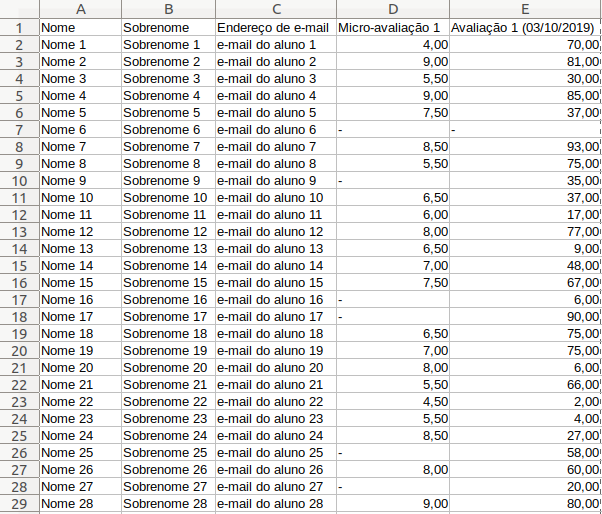
\includegraphics[height=0.6\textwidth]{./dados/figuras/planilha-notas-2}
    \fonte{Autoria Própria}
    \label{fig:planilha-notas}
\end{figure}

Para a submissão das faltas é aceito o formato disponibilizado pelas planilhas exportadas pelo sistema acadêmico da UTFPR. 
Neste arquivo é disposto um código identificador ou Registro Acadêmico (R.A.), nome do aluno, total de faltas e colunas que representam cada um dos dias de aula corridos no período letivo, com o número de ausências de cada aluno em cada um desses dias.

O formato da planilha de faltas disponibilizada atualmente pelo sistema acadêmico da UTFPR é apresentado na figura \ref{fig:planilha-faltas}, mas em alguns casos estas são exportadas com sua estrutura semelhante a apresentada na figura \ref{fig:planilha-faltas-2}. 
A plataforma desenvolvida também está preparada para receber dados neste formato e ao carregar uma planilha neste padrão ele internamente realizará a re-estruturação desta para o formato apresentado na figura \ref{fig:planilha-faltas} e em seguida a extração e persistência dos dados.

\begin{figure}[!htb]
    \centering
    \caption{Modelo de planilha com faltas exportada do sistema acadêmico da UTFPR}
    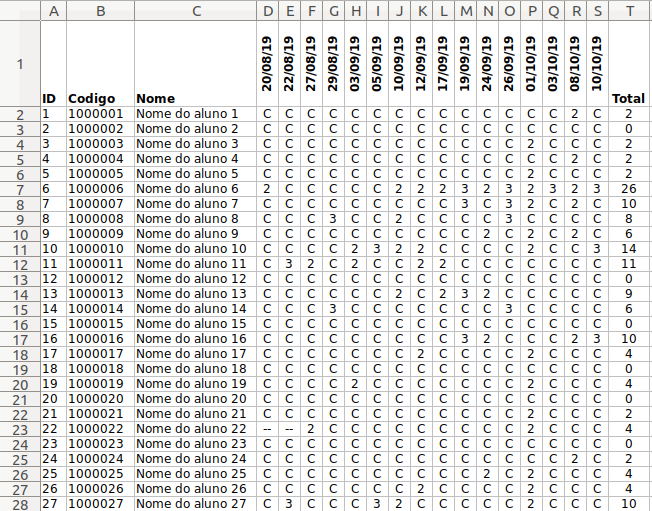
\includegraphics[height=0.6\textwidth]{./dados/figuras/planilha-faltas}
    \fonte{Autoria Própria}
    \label{fig:planilha-faltas}
\end{figure}

\begin{figure}[!htb]
    \centering
    \caption{Modelo alternativo de planilha com faltas exportada pelo sistema acadêmico da UTFPR}
    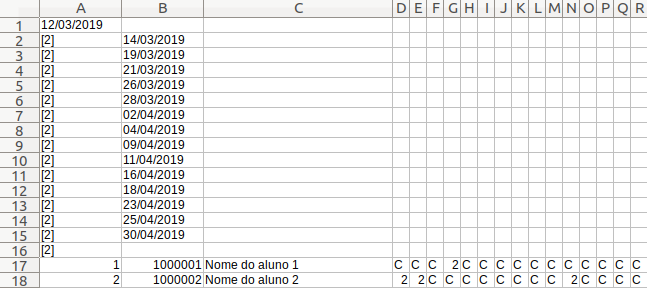
\includegraphics[height=0.35\textwidth]{./dados/figuras/planilha-faltas-2}
    \fonte{Autoria Própria}
    \label{fig:planilha-faltas-2}
\end{figure}

Para o upload de dados de notas e faltas, obtidos no Moodle e sistema acadêmico, respectivamente, é necessário que ambas as planilhas estejam consolidadas em somente um arquivo, como abas, como apresentado na figura \ref{fig:planilha-abas-selecionadas}.
Por mais que reflita em uma etapa a mais de trabalho manual demandado do usuário, isto é usado como um recurso para evitar o upload de notas e de faltas de períodos divergentes ou planilhas que não estão sincronizadas entre si quanto a data corrente do periodo letivo. 
Por exemplo o upload de notas dos alunos até certa data do período letivo e ao mesmo tempo upload das faltas referentes a uma data posterior.

Os nomes das abas não influenciam na importação dos dados, contanto que a ordem delas seja a mesma da apresentada na figura \ref{fig:planilha-abas-selecionadas}, sendo a primeira aba destinada às notas e a segunda aba destinada às faltas dos alunos.

\begin{figure}
\centering
\caption{Planilha de dados com notas e faltas separadas por abas}
\begin{subfigure}{.4\textwidth}
  \centering
  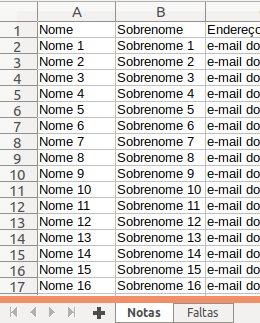
\includegraphics[width=.9\linewidth]{./dados/figuras/planilha-selecionado-notas}
  \end{subfigure}%
\begin{subfigure}{.4\textwidth}
  \centering
  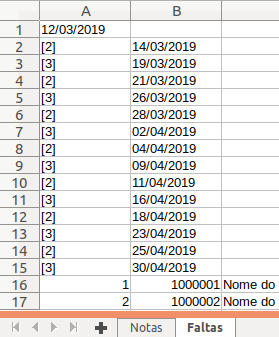
\includegraphics[width=.9\linewidth]{./dados/figuras/planilha-selecionado-faltas}
\end{subfigure}
\label{fig:planilha-abas-selecionadas}
\end{figure}

Além destes dois arquivos, foi considerado como fonte de dados a plataforma URI, citada anteriormente na subseção \ref{sec:entendimentoNegocio2}, desta forma o sistema desenvolvido também possibilita o envio de planilhas com dados da plataforma URI.

\begin{figure}[!htb]
    \centering
    \caption{Modelo de planilha com dados exportada pela plataforma URI}
    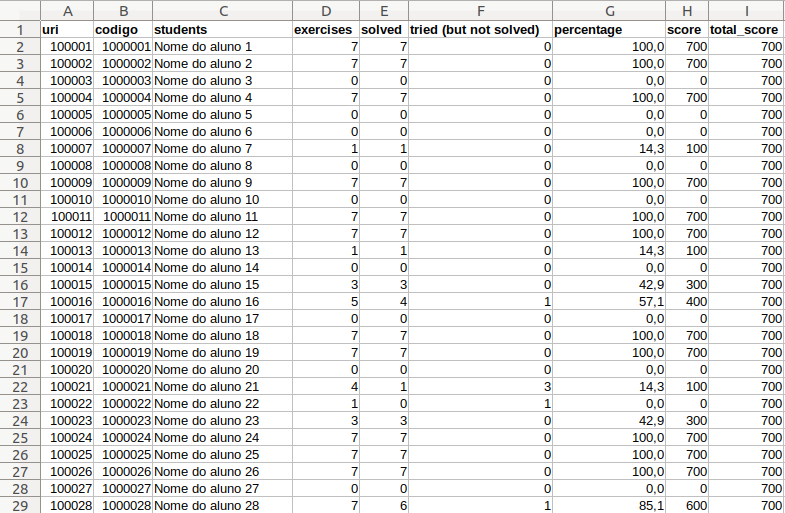
\includegraphics[height=0.6\textwidth]{./dados/figuras/planilha-uri}
    \fonte{Autoria Própria}
    \label{fig:planilha-uri}
\end{figure}

O sistema foi configurado para permitir o upload de arquivos gerados com extensão \textit{xls} e \textit{xlsx}, formatos padrões utilizados pelo gerenciador de planilhas \textit{Excel}, da Microsoft, \textit{ods}, formato utilizado pelo software open-source \textit{LibreOffice Calc}, e \textit{csv}, formato bastante utilizado por sistemas de exportação de texto formatado por vírgulas.

A plataforma também é capaz de distinguir os nomes das colunas, então é recomendado que estes sejam descritos conforme os apresentados nas figuras \ref{fig:planilha-notas}, \ref{fig:planilha-faltas} (caso possível) ou \ref{fig:planilha-faltas-2} e \ref{fig:planilha-uri}. 
Algumas alternativas de nomes de colunas também podem ser utilizadas, como Trabalho 1 ou Atividade 1 ao invés de Micro-avaliação 1, e Prova 1 ao invés de Avaliação 1. 
É importante a inserção das datas das avaliações em seu nome na atividade do Moodle, por exemplo Avaliação 1 - 03/10/2019 ou Avaliação 1 (03/10/19), para que seja possível associar as faltas até esta data. 
Não é necessário seguir um padrão específico de separador entre o nome da atividade e a data, uma vez que é utilizado uma expressão regular para capturar a data no título, caso existente.

Lembrando que todas as planilhas citadas anteriormente são disponibilizadas pelos seus respectivos sistemas, assim a coleta destes e inserção no sistema de predição ainda é feita de forma manual, mas o trabalho manual de manipulação dos dados das planilhas é eliminado.

Após a aquisição dos dados iniciais, que foram utilizados para estruturar a aplicação, foi-se identifica a relação entre os tipos de planilhas inseridos por meio do código identificador do aluno.
Foi possível verificar também que a planilha de notas pode contém valores faltantes, campos vazios ou com caracteres especiais como o ``-'' (traço). 
Analisando-o pode-se perceber que estes pertencem a alunos que não realizaram provas ou atividades, e estes podem ser substituídos por um valor padrão, neste caso o valor 0 (zero).

Foi-se então realizada uma análise dos dados, considerando a princípio as notas das avaliações, a realização de trabalho, a resolução de exercícios do URI e as frequências dos alunos. 
Com isto gerou-se alguns gráficos.

A figura \ref{fig:analise-1} mostra um gráfico de dispersão contendo no eixo horizontal as frequências dos alunos e no eixo vertical a nota média destes. 
Usou como variável também a realização ou não de trabalhos, os pequenos círculos ilustram os alunos que deixaram de realizar algum dos trabalhos, enquanto que os símbolos em X ilustram os alunos que realizaram todas as atividades. 
Pode-se perceber uma concentração de maiores notas quando os alunos possuem maiores frequências nas aulas e a realização dos trabalhos propostos torna ainda mais evidente esta relação.

\begin{figure}[!htb]
    \centering
    \caption{Gráfico de dispersão com as frequências e notas dos alunos, considerando a realização de todos os trabalhos}
    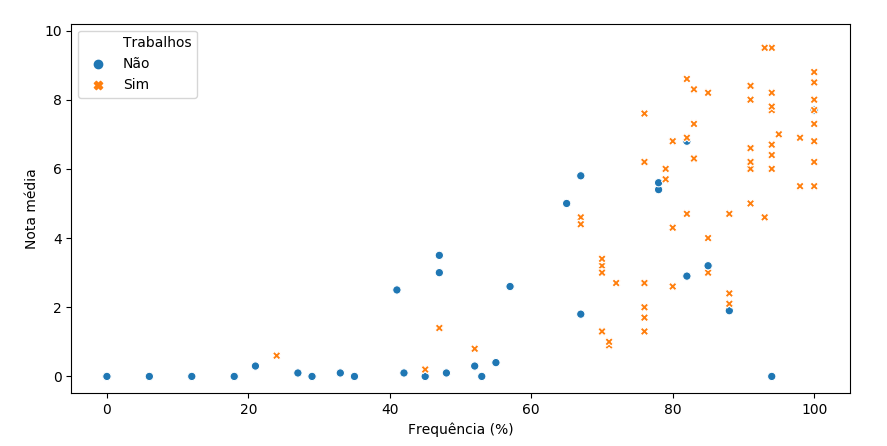
\includegraphics[width=1\textwidth]{./dados/figuras/analise/grafico1}
    \fonte{Autoria Própria}
    \label{fig:analise-1}
\end{figure}

A figura \ref{fig:analise-2} apresenta um gráfico com dois \textit{subplots}, no eixo horizontal de ambos é apresentado a nota obtida, já o eixo vertical mostra a quantidade de alunos com esta nota.
O \textit{plot} da esquerda é composto pelos alunos que realizaram todos os trabalhos e o da direita pelos alunos que não realizaram algum dos trabalhos. 
Pode-se observar uma maior concentração de alunos com boas notas na ilustração da esquerda, já no da direita a distribuição das notas diferente, não havendo notas maiores do que oito. 
Neste o número de alunos com nota zero ultrapassa oito, mas para melhor comparação foi-se limitado o eixo vertical de ambos os gráficos neste valor.

\begin{figure}[!htb]
    \centering
    \caption{Gráficos de barra com as quantidades de alunos por faixa de notas}
    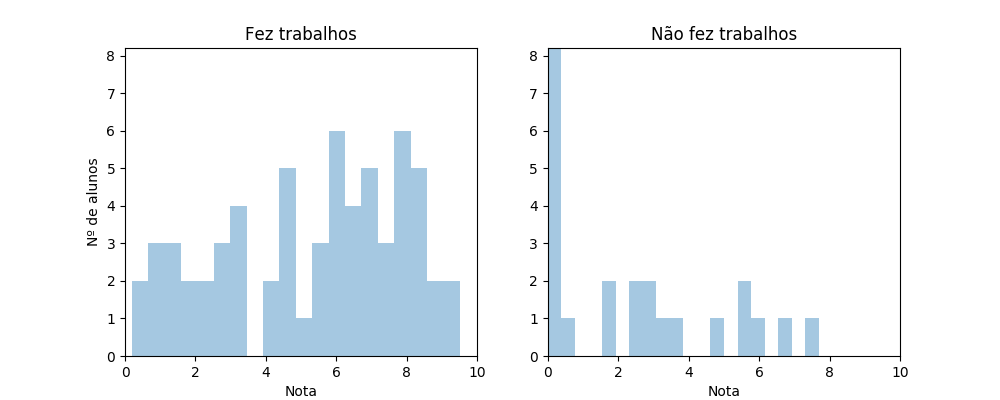
\includegraphics[width=1\textwidth]{./dados/figuras/analise/grafico2}
    \fonte{Autoria Própria}
    \label{fig:analise-2}
\end{figure}

Já as figuras \ref{fig:analise-3} e \ref{fig:analise-4} mostram as notas e o número de alunos mas segmentando-as pela resolução dos exercícios do URI. 
Para ambas, a ilustração da esquerda mostra os alunos que resolveram 50\% ou mais dos exercícios propostos, enquanto nos gráficos da direita é descrito os alunos que resolveram menos de 50\% dos exercícios.
Ao averiguá-los é possível perceber que a realização dos trabalhos em conjunto da resolução dos exercícios do URI foi o padrão seguido que apresentou melhores resultados, neste a distribuição das notas ficou mais concentrada entre 5,5 e 9,5.

Em contrapartida, para os alunos que não realizaram trabalhos nem exercícios do URI a concentração se deu entre 0 e 0,5, neste também o gráfico foi limitado ao valor cinco, mas a quantidade real de alunos com nota zero foi 16.

Para a concepção destes gráficos foram utilizados os dados de todos os alunos e então é importante observar que há a possibilidade de que uma parcela considerável das notas mais baixas seja referente a alunos que nunca compareceram as aulas ou em pouco tempo deixaram de frequentá-las.

\begin{figure}[!htb]
    \centering
    \caption{Gráficos de barra com as quantidades de alunos que realizaram todos os trabalhos por faixa de notas, considerando os exercícios do URI}
    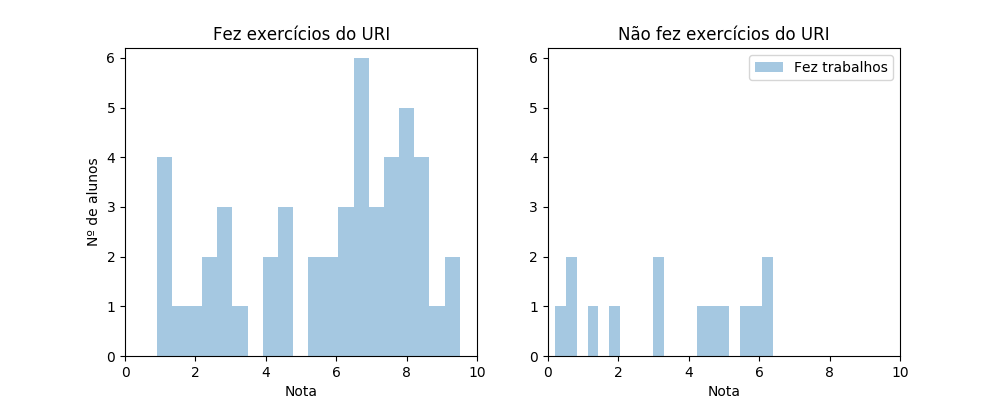
\includegraphics[width=1\textwidth]{./dados/figuras/analise/grafico3}
    \fonte{Autoria Própria}
    \label{fig:analise-3}
\end{figure}

\begin{figure}[!htb]
    \centering
    \caption{Gráficos de barra com as quantidades de alunos que deixaram de realizar algum trabalho por faixa de notas, considerando os exercícios do URI}
    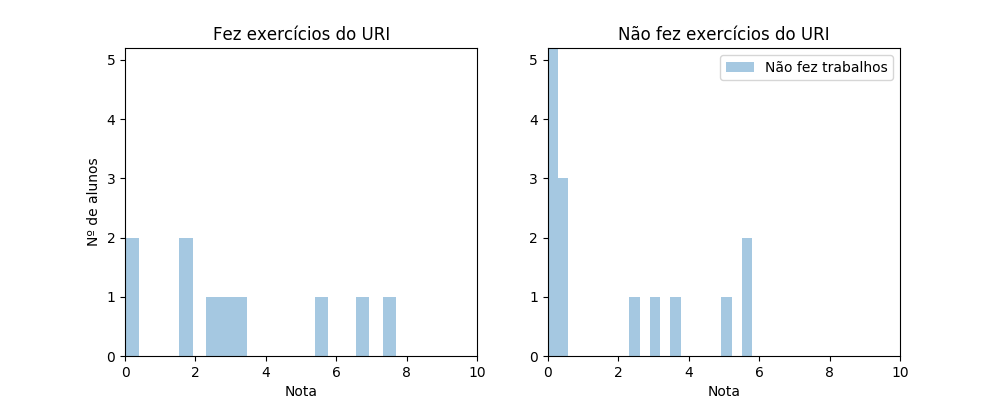
\includegraphics[width=1\textwidth]{./dados/figuras/analise/grafico4}
    \fonte{Autoria Própria}
    \label{fig:analise-4}
\end{figure}


\section{PREPARAÇÃO DOS DADOS}

Como já descrito no tópico \ref{sssec:preparacaoDados}, esta etapa consiste em tratar os dados a fim de dispor o conjunto de dados que será utilizado para o processamento e construção do modelo de mineração de dados, bem como para outros fins, como para apresentação e construção dos gráficos.

Nesta fase foram criados \textit{scripts} para formatação dos dados, a fim de permitir o uso destes para o processamento sem ruídos, incoerências ou redundâncias, reduzindo assim as chances de resultados anômalos.

Inicialmente implementou-se um \textit{script} no \textit{back-end} em Node.js, que efetua a formatação dos dados iniciais para um formato mais adequado para a construção de gráficos e uso nos modelos de predição.
Neste \textit{script} os dados das planilhas são convertidos para o formato JSON utilizando a biblioteca \textit{SheetJS}, que torna mais simples a manipulação dos dados, já que o formato é nativo o linguagem de programação \textit{Typescript}, utilizada no projeto.
Em seguida as notas e frequências inicialmente armazenadas em tipo texto são convertidas para valores numéricos, e as letras que eram utilizadas para representar o status de presença do aluno foram convertidas também para valores numéricos.
Neste contexto a letra C representa os alunos presentes e a letra D representam que este havia sido dispensado com alguma justificativa, como a participação em algum evento ocorrente na universidade, e por isso não havia a contagem de faltas.

Como pode-se observar, as etapas do modelo CRISP-DM são nitidamente conectadas, visto que este último tratamento citado envolve também a etapa de entendimento dos dados. 

A figura \ref{fig:dados-notas-pos} apresenta a estrutura final dos dados de notas, que compõe além das notas alguns outros dados essenciais para o trabalho, que serão melhor detalhados posteriormente. 
A estrutura dos dados é composta pelos seguintes campos:

\begin{itemize}[topsep=5pt]
    \item \textbf{\_id:} ID de Objeto único gerado para este documento pelo MongoDB, ou seja, é a chave primária deste registro no banco de dados;
    \item \textbf{code:} Código identificador/R.A. do aluno;
    \item \textbf{course\_unit:} Código da disciplina ao qual o aluno está vinculado e as notas são referentes;
    \item \textbf{name:} Contém o nome completo do aluno;
    \item \textbf{email:} Campo que contém o e-mail do aluno;
    \item \textbf{attendance:} Contém a frequência, em percentual, do aluno para a disciplina associada a este registro, é calculada com base na quantidade de aulas dadas;
    \item \textbf{current\_grade:} Contém a nota atual do aluno, é calculada com base no peso aplicado para avaliações e atividades;
    \item \textbf{feedbacks:} Este campo é destinado a conter a lista de notificações enviadas por e-mail ao aluno pela plataforma, juntamente às justificativas, ou \textit{feedbacks}, enviados pelo aluno para cada e-mail recebido.
\end{itemize}

Os campos a seguir são gerados dinamicamente conforme as colunas existentes na planilha origem do dado, podendo assim haver um ou mais campos para notas de avaliação, gerando assim campos \textit{gradeN}, sendo N o número de cada avaliação.
Bem como é possível não haver campos para datas de prova, caso esta não esteja presente no cabeçalho da coluna na planilha.
A mesma lógica se aplica para as atividades, podendo assim haver zero, uma ou múltiplas atividades realizadas pelo aluno.

\begin{itemize}[topsep=5pt]
    \item \textbf{grade1:} Contém a nota obtida pelo aluno para a 1ª avaliação da disciplina associada a este registro;
    \item \textbf{grade1\_date:} Contém a data da 1ª avaliação;
    \item \textbf{micro\_grade1:} Contém a nota obtida pelo aluno para a 1ª atividade realizada na disciplina.
\end{itemize}

\begin{figure}[!htb]
    \centering
    \caption{Fragmento do conjunto de dados de notas após preparação}
    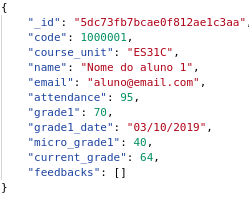
\includegraphics[height=0.35\textwidth]{./dados/figuras/dados-notas-pos}
    \fonte{Autoria Própria}
    \label{fig:dados-notas-pos}
\end{figure}

Então as faltas, que são apresentadas por aula dada, são transformadas para um formato acumulativo, o que facilita também a construção dos gráficos.
Todas estas transformações são realizadas sobre dados no formato apresentado anteriormente na figura \ref{fig:planilha-faltas}, e o resultado é apresentado na figura \ref{fig:dados-faltas-pos}, que exibe o conjunto de dados pós-preparação.

Por fim os dados são armazenados no banco de dados com o uso do \textit{Mongoose}, e a figura \ref{fig:dados-faltas-pos} mostra a estrutura de dados JSON no formato final, que é composta pelos seguintes campos:

\begin{itemize}[topsep=5pt]
    \item \textbf{\_id:} ID de Objeto único gerado para este documento pelo MongoDB, ou seja, é a chave primária deste registro no banco de dados;
    \item \textbf{code:} Código identificador/R.A. do aluno; 
    \item \textbf{course\_unit:} Código da disciplina ao qual o aluno está vinculado e as faltas são referentes;  
    \item \textbf{active:} Campo booleano utilizado para definir o status do aluno na disciplina, caso a frequência seja verificada abaixo de 25\% do total de aulas o aluno é considerado inativo, caso contrário é ativo;
    \item \textbf{total:} Contém o número total de faltas do aluno para a disciplina relacionada no momento do upload dos dados; 
    \item \textbf{absences:} É um campo do tipo Array, que contém um objeto para cada dia de aula dada até o momento. Os campos de cada objeto representam a data da aula e o número de faltas acumuladas do aluno ao decorrer das aulas.
    \item \textbf{id:} Campo opcional, é populado caso a planilha carregada possua uma coluna nomeada como ID e é utilizado para ordenação.
\end{itemize}

\begin{figure}[!htb]
    \centering
    \caption{Fragmento do conjunto de dados de faltas após preparação}
    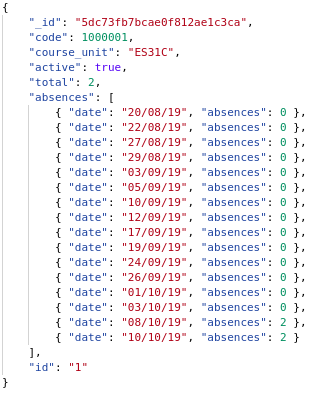
\includegraphics[height=0.65\textwidth]{./dados/figuras/dados-faltas-pos}
    \fonte{Autoria Própria}
    \label{fig:dados-faltas-pos}
\end{figure}

A figura \ref{fig:dados-uri-pos} mostra parcela dos dados após a preparação realizada ao receber a planilha de dados exportada pela plataforma URI.
Estes são compostos pelos seguintes campos:

\begin{itemize}[topsep=5pt]
    \item \textbf{\_id:} ID de Objeto único gerado para este documento pelo MongoDB, ou seja, é a chave primária deste registro no banco de dados;
    \item \textbf{code:} Código identificador/R.A. do aluno; 
    \item \textbf{course\_unit:} Código da disciplina ao qual o aluno está vinculado e os exercicios do URI são referentes; 
    \item \textbf{name:} Contém o nome completo do aluno;
    \item \textbf{exercises:} Contém a quantidade de exercícios aos quais o aluno solucionou completa ou parcialmente;
    \item \textbf{solved:} Contém a quantidade de exercícios que o aluno finalizou corretamente;
    \item \textbf{tried:} Contém a quantidade de exercícios que o aluno tentou solucionar, mas não os finalizou;
    \item \textbf{percentage:} Contém a porcentagem de exercícios solucionados de forma integral;
    \item \textbf{total:} Contém a quantidade total de exercícios para a lista em questão;
    \item \textbf{exam:} Contém a referência da avaliação a qual este registro é associado.
\end{itemize}

\begin{figure}[!htb]
    \centering
    \caption{Fragmento do conjunto de dados obtidos na plataforma URI após preparação}
    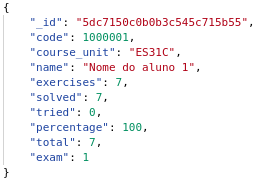
\includegraphics[height=0.32\textwidth]{./dados/figuras/dados-uri-pos}
    \fonte{Autoria Própria}
    \label{fig:dados-uri-pos}
\end{figure}

Vale ressaltar que para um volume pequeno de dados, estas alterações poderiam ser efetuadas manualmente sem grande demanda de tempo, mas para um volume maior de dados, como possivelmente esperado no uso da plataforma desenvolvida, se faz necessário a criação de rotinas de preparação de dados para a realização destas tarefas.
Ressalta-se também que este trabalho tem como objetivo automatizar o maior número possível de tarefas, demandando o mínimo de atuação manual por conta do usuário após a aquisição dos dados.

\section{MODELAGEM}
\label{sec:modelagem}
Uma vez realizada a preparação dos dados, é possível seguir para a implementação dos modelos de mineração de dados.

Neste trabalho foram utilizados três algoritmos de \textit{machine learning} (ML), ou aprendizado de máquina supervisionados, são estes a regressão linear, o \textit{random forest} e o \textit{gradient boosting}, descritos na seção \ref{sec:mineracaoDados}, que descreve a mineração de dados.
Como um dos objetivos deste trabalho é predizer o desempenho dos alunos com base em suas notas e faltas, os algoritmos foram utilizados como técnicas de regressão, mesmo o \textit{random forest} e o \textit{gradient boosting} possuindo a capacidade de atuar como técnicas de classificação de dados.

Desta forma foram implementados os algoritmos com o auxílio das bibliotecas de aprendizado de máquina \textit{Scikit-Learn} e de manipulação de dados \textit{Pandas}.

O trecho de código apresentado na listagem \ref{cod:treinamentoModelos} é utilizado para treinar os modelos de ML citados.
O conjunto de dados foi dividido em subconjuntos de treinamento e teste utilizando a razão 80\%/20\%.
O modelo baseado em \textit{Gradient Boosting} foi gerado com 400 estimadores, que internamente se traduzem em árvores de regressão em formato \textit{boosting}, descrito na \ref{ssec:gradientBoosting}, com profundidade máxima igual a cinco e empregando a função erro \textit{least squares}, ou mínimos quadrados.
O modelo que utiliza \textit{Random Forest} foi gerado utilizando também 400 estimadores, que desta vez geram árvores de regressão em formato \textit{bagging}, descrito na \ref{ssec:randomForest}.
Já o algoritmo de regressão linear não demanda nenhum argumento específico para a criação e treinamento de modelos.

\begin{lstlisting}[caption={Trecho de código para treinamento dos modelos de ML}, label={cod:treinamentoModelos}]

## Divisao do conjunto de dados em treinamento (80%) e teste (20%).
x_train, x_test, y_train, y_test = train_test_split(data.values, labels.values, test_size=0.2, random_state=42)

## Gradient Boosting Model
gradient_model = GradientBoostingRegressor(n_estimators=400, max_depth=5, loss='ls')
gradient_model.fit(x_train, y_train)

## Random Forest Model
random_forest = RandomForestRegressor(n_estimators=400)
random_forest.fit(x_train, y_train)

## Linear Regression Model
linear_regression = LinearRegression()
linear_regression.fit(x_train, y_train)
\end{lstlisting}

A biblioteca \textit{Scikit-learn} possibilita extrair a importância, ou peso, de cada \textit{feature} dos modelos treinados com os algoritmos \textit{Gradient Boosting} e \textit{Random Forest}, ou seja, é possível obter a porcentagem que cada variável utilizada no treinamento influencia nas estimativas retornadas pelos modelos.
A tabela \ref{tab:importanciaGradient} mostra a importância das \textit{features} no modelo treinado com o algoritmo \textit{Gradient Boosting}, considerando dados de turmas que realizaram duas avaliações e três atividades/trabalhos.
A tabela \ref{tab:importanciaRandom} também apresenta a importância das \textit{features}, entretanto para o modelo treinado com o algoritmo \textit{Random Forest}.

\begin{table}[!htb]
    \centering
    \caption{Importância das \textit{features} para o modelo treinado com \textit{Gradient Boosting}}
    \begin{tabular}{@{}cc@{}}
        \hline
        \textbf{ Feature } & \textbf{ Importância } \\ \hline
        grade2  & 79,7\% \\
        micro\_grade1  & 8,9\% \\
        grade1  & 7,8\% \\
        attendance  & 3,2\% \\
        micro\_grade3  & 0,4\% \\
        micro\_grade2  & 0,0\% \\ \bottomrule
    \end{tabular}
    \label{tab:importanciaGradient}
\end{table}

\begin{table}[!htb]
    \centering
    \caption{Importância das \textit{features} para o modelo treinado com \textit{Random Forest}.}
    \begin{tabular}{@{}cc@{}}
        \hline
        \textbf{ Feature } & \textbf{ Importância } \\ \hline
        grade2  & 55,7\% \\
        grade1  & 22,3\% \\
        attendance  & 14,5\% \\
        micro\_grade1  & 5,2\% \\
        micro\_grade3  & 1,7\% \\
        micro\_grade2  & 0,6\% \\ \bottomrule
    \end{tabular}
    \label{tab:importanciaRandom}
\end{table}

Já a tabela \ref{tab:importanciaUmaProva} apresenta os pesos das \textit{features} para ambos os modelos considerando somente uma avaliação e uma atividade/trabalho, mas com atividades da plataforma URI realizadas pela turma, o campo \textit{percentage} no treinamento do modelo contém a porcentagem de exercícios solucionados ou que houve tentativa de resolução pelo aluno.
Desta forma as únicas \textit{features} disponíveis para a criação do modelo foram a nota da avaliação, a nota da atividade e a frequência do aluno.

\begin{table}[!htb]
    \centering
    \caption{Importância das \textit{features}, considerando somente uma avaliação e um trabalho, para modelos treinados com \textit{Gradient Boosting} e \textit{Random Forest}.}
    \begin{tabular}{@{}ccc@{}}
    \textbf{} & \multicolumn{2}{c}{\textbf{Importância}} \\ \midrule
    \textbf{Feature} & \textbf{Gradient B.} & \textbf{Random F.} \\ \midrule
        grade1  & 89,6\%  & 92,7\% \\
        micro\_grade1  & 8,2\%  & 5,1\% \\
        attendance  & 1,2\%  & 1,1\% \\ 
        percentage  & 1,0\%  & 1,1\% \\ \bottomrule
    \end{tabular}
    \label{tab:importanciaUmaProva}
\end{table}

Como apresentado na \ref{sec:entendimentoDados2}, ao realizar o upload da planilha de faltas são salvas também as presenças dos alunos a cada aula dada no período letivo. então construiu-se modelos com base nos dois algoritmos utilizados anteriormente considerando as datas de cada aula, a fim de avaliar a importância individual das aulas nas predições. 
A tabela \ref{tab:importanciaComDatas} apresenta os pesos retornados pelos dois modelos, nesta as datas são representadas pelos campos date\_N, onde N é sequencialmente o número da aula dada. 
A título de exemplificação, ao realizar um paralelo com os dados já apresentados nas seções de entendimento e preparação dos dados, os campos \textit{date\_1} e \textit{date\_2} da tabela \ref{tab:importanciaComDatas} remetem respectivamente às datas 20/08/19 e 22/08/19 da figura \ref{fig:dados-faltas-pos}, e assim sucessivamente.

\begin{table}[!htb]
    \centering
    \caption{Importância das \textit{features}, considerando datas, para os modelos treinados com \textit{Gradient Boosting} e \textit{Random Forest}.}
    \begin{tabular}{@{}ccc@{}}
    % \cmidrule(l){2-3}
    \textbf{} & \multicolumn{2}{c}{\textbf{Importância}} \\ \midrule
    \textbf{Feature} & \textbf{Gradient B.} & \textbf{Random F.} \\ \midrule
        grade1 & 89,7\%  &  91,3\% \\
        micro\_grade1  & 8,4\%  &  7,6\% \\
        attendance  & 0,8\%  &  1,0\% \\
        date\_13  & 0,2\%  &  0,1\% \\
        date\_12  & 0,2\%  &  0,1\% \\ 
        date\_11  & 0,1\%  &  0,0\% \\
        date\_8  & 0,1\%  &  0,0\% \\
        date\_7  & 0,1\%  &  0,0\% \\
        date\_5  & 0,1\%  &  0,0\% \\
        date\_2  & 0,1\%  &  0,0\% \\
        date\_6  & 0,0\%  &  0,0\% \\
        date\_4  & 0,0\%  &  0,0\% \\
        date\_9  & 0,0\%  &  0,0\% \\
        date\_10  & 0,0\%  &  0,0\% \\
        date\_3  & 0,0\%  &  0,0\% \\
        date\_1  & 0,0\%  &  0,0\% \\
        date\_14  & 0,0\%  &  0,0\% \\
        date\_15  & 0,0\%  &  0,0\% \\
        \bottomrule
    \end{tabular}
    \label{tab:importanciaComDatas}
\end{table}

O algoritmo de regressão linear não possui o artificio de identificação das importâncias como os outros, porém ele permite obter os coeficientes determinados pelo modelo para a composição da equação linear que descreve os dados.
Estes coeficientes considerando o conjunto de dados com duas avaliações são apresentados na tabela \ref{tab:coef-linear}.

\begin{table}[!htb]
    \centering
    \caption{Coeficientes definidos pelo modelo de regressão linear considerando duas avaliações}
    \begin{tabular}{@{}cc@{}}
        \hline
        \textbf{ Feature } & \textbf{ Coeficiente } \\ \hline
        grade2  & 0,473 \\
        grade1  & 0,407 \\
        micro\_grade1  & 0,048 \\
        micro\_grade3  & 0,041 \\
        micro\_grade2  & 0,027 \\
        attendance  & 0,008 \\
        percentage  & -0,004 \\ \bottomrule
    \end{tabular}
    \label{tab:coef-linear}
\end{table}

% Ao final será verificado se às questões construídas na subseção \ref{sec:entendimentoNegocio2} podem ser respondidas e se os resultados são satisfatórios. Se forem, estes podem ser levados à etapa de implantação.

\section{IMPLEMENTAÇÃO}
\label{sec:implementacao}

Para esta etapa do trabalho, foi-se então construído um sistema web, do qual tem como finalizar permitir o acesso aos dados, gráficos e artifícios implementados.
O sistema é composto por seis páginas, sendo que quatro destas estão dispostas no menu lateral da plataforma, são estas: \textbf{Dashboard}, \textbf{Configurações}, \textbf{Upload de Dados},  e \textbf{Lista}.
A quinta página é a de \textbf{Detalhes do Estudante} e pode ser acessada pelo Dashboard ou pela Lista ao clicar em uma das linhas das listas de alunos. 
E a última página é a página de \textbf{Feedback} acessada somente pelos alunos por meio de um link exclusivo. Este recurso será melhor explorado posteriormente.

A figura \ref{fig:diagrama-1} apresenta as chamadas realizadas entre os componentes do sistema quando realizado o upload de uma planilha. 
Inicialmente o usuário carrega a planilha por meio da página de upload de dados do sistema, essa é enviada ao \textit{back-end} escrito em Node.js, que por sua vez realiza a manipulação das planilhas, transformação em formato JSON e a preparação dos dados. 
Em seguida os dados formatados são inseridos na base de dados MongoDB com auxílio do \textit{Mongoose}.

\begin{figure}[htb]
    \centering
    \caption{Fluxo de interações entre os componentes do sistema no upload de dados}
    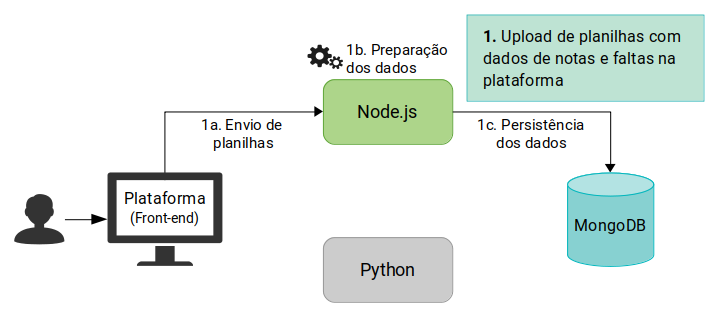
\includegraphics[height=0.35\textwidth]{./dados/figuras/diagrama1}
    \fonte{Autoria Própria}
    \label{fig:diagrama-1}
\end{figure}

Já para chamadas requisitando dados, a figura \ref{fig:diagrama-2} ilustra o processo, que pode ser realizado por dois caminhos distintos:

\begin{enumerate}[topsep=5pt]
    \item \textbf{Dados em geral:} Estes são utilizados para apresentação, listagem ou para construção de gráficos no \textit{front-end}, e para este tipo de dados são realizadas chamadas ao \textit{back-end} Node.js, que busca os dados no BD, transforma-os conforme a demanda específica, realiza os cálculos necessários para apresentação, como a média de faltas da turma para cada aula do período letivo e a média das notas dos alunos em cada disciplina, e então retorna-os.
    \item \textbf{Predições:} Para predições a chamada é enviada para o \textit{back-end} em Python, que busca os dados necessários no BD, reformata-os para o uso com os modelos de machine learning criados e citados anteriormente, busca o modelo correto a ser carregado com base nos dados atuais do aluno e então executa os algoritmos, retornando os resultados. 
\end{enumerate}

\begin{figure}[!htb]
    \centering
    \caption{Fluxo de interações entre os componentes do sistema em requisições solicitando dados e predições}
    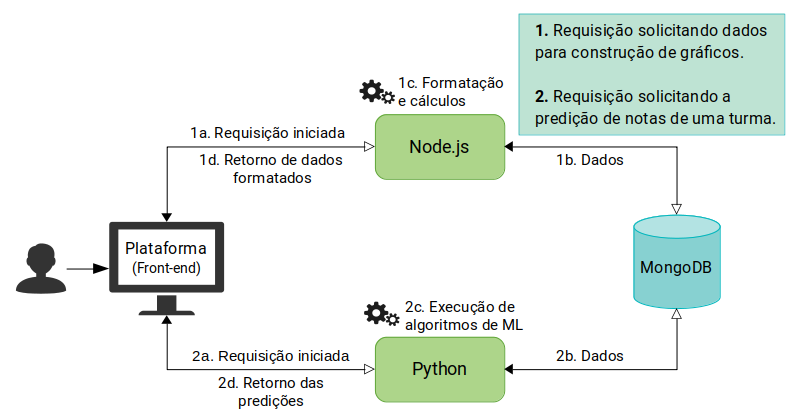
\includegraphics[height=0.45\textwidth]{./dados/figuras/diagrama2}
    \fonte{Autoria Própria}
    \label{fig:diagrama-2}
\end{figure}

\subsection{Dashboard}
\label{ssec:dashboard}

A página inicial da plataforma consiste do Dashboard. 
Este é apresentado nas figuras \ref{fig:dashboard-1} e \ref{fig:dashboard-2}.
Os indicadores apresentados no topo nas cores verde, amarelo e vermelho levam em conta a nota dos alunos e mostram o número de alunos em situações tendenciosas a aprovação, com notas medianas e com um risco maior de reprovação, respectivamente.
Para esta separação foram criados dois \textit{thresholds} e com base em um sistema de notas de 0 a 100 foram sugeridas as seguintes regras:
\begin{itemize}[topsep=5pt]
    \item \textbf{Aprovado:} Nota prevista maior ou igual a 70;
    \item \textbf{Limiar:} Nota prevista entre 50 e 70;
    \item \textbf{Alto risco:} Nota prevista abaixo de 50;
\end{itemize}

Estas regras foram criadas como uma forma de priorização de perfis de alunos na realização de ações, ou seja, os usuários do sistema, interessados em interagir com os alunos ou desenvolver mecanismos para prevenir a retenção podem iniciar com o perfil de \textit{alto risco} como seu público alvo. 
Da mesma pode-se tomar diferentes ações com o perfil \textit{limiar}, uma vez que estes alunos, em tese, demandam de menos esforço para garantir a aprovação nas disciplinas.

Localizados na direita superior da figura \ref{fig:dashboard-1} tem-se o número total de alunos cadastrados na plataforma e uma caixa de seleção flutuante, que permite selecionar uma das disciplinas cadastradas ou manter a opção Todas as Disciplinas para visualizar os dados de forma geral.

Ainda na figura \ref{fig:dashboard-1} tem-se o gráfico temporal de faltas dos alunos de uma turma, comparando-as com o limite parcial para reprovação por faltas da UTFPR, atualmente de 25\% do total de aulas dadas no período letivo.
O eixo horizontal é composto pelas datas dos dias de aula até o momento em que os dados foram carregados na ferramenta, e o eixo vertical mostra a média das ausências absolutas em cada aula dos alunos de uma turma, neste caso da disciplina ES31C - Laboratório de Informática.

Para obter números mais práticos e condizentes com a realidade, no cálculo desta média não são considerados os alunos inativos, ou seja, que possuem menos de 25\% de frequência, pois a inserção de dados de alunos que cancelaram sua matrícula, nunca foram as aulas ou foram somente nas aulas iniciais poderia influenciar negativamente nos números gerais. 
Estes alunos ainda podem ser analisados individualmente, porém para efeitos de cálculos coletivos eles não são considerados.

A escolha do \textit{threshold} para determinar se um aluno é ativo ou inativo foi estipulada de forma empírica observando os dados disponíveis, mas caso seja observado ao longo do tempo um valor mais preciso para descrever esse comportamento, o \textit{threshold} poderia ser alterado.

\begin{figure}[!htb]
    \centering
    \caption{Fragmento superior do dashboard}
    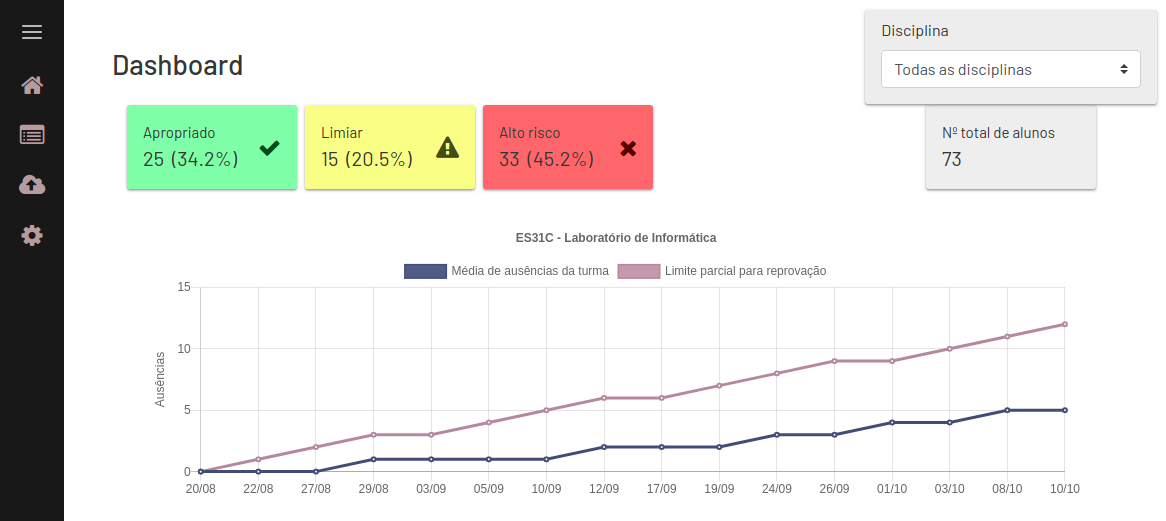
\includegraphics[width=1\textwidth]{./dados/figuras/sistema/sistema-dashboard-1}
    \fonte{Autoria Própria}
    \label{fig:dashboard-1}
\end{figure}

A figura \ref{fig:dashboard-2} apresenta a segunda parte do dashboard. 
O primeiro gráfico apresentado nesta tela tem como objetivo mostrar a relação entre a frequência e notas dos alunos, caso exista, levando em conta se estes realizaram atividades/trabalhos ou não.
O eixo horizontal contém os percentuais de frequência dos alunos cadastrados, confrontando-as com as notas atuais dos mesmos no eixo vertical. 
Os pontos de cor azul ilustram os alunos que entregaram todas as atividades, independente das notas obtidas. 
Já os pontos avermelhados ilustram alunos que deixaram de realizar pelo menos uma das atividades.
Para a composição deste gráfico as atividades realizadas com nota igual a zero são consideradas como não realizadas.

A tabela à direita do gráfico citado anteriormente mostra os principais pontos de atenção, ou seja, a lista dos alunos com menores notas entre os cadastrados, descartando da listagem os alunos considerados inativos. Ao clicar em um dos alunos é apresentada a tela de detalhes do aluno.

Em seguida são apresentados os gráficos de barras e de rosca, que ilustram a proporção de alunos em situação de aprovação, média e reprovação. O primeiro segmenta os dados por disciplina, enquanto o segundo procura mostrar uma visão geral da situação em todas as disciplinas cadastradas.

\begin{figure}[!htb]
    \centering
    \caption{Fragmento inferior do dashboard}
    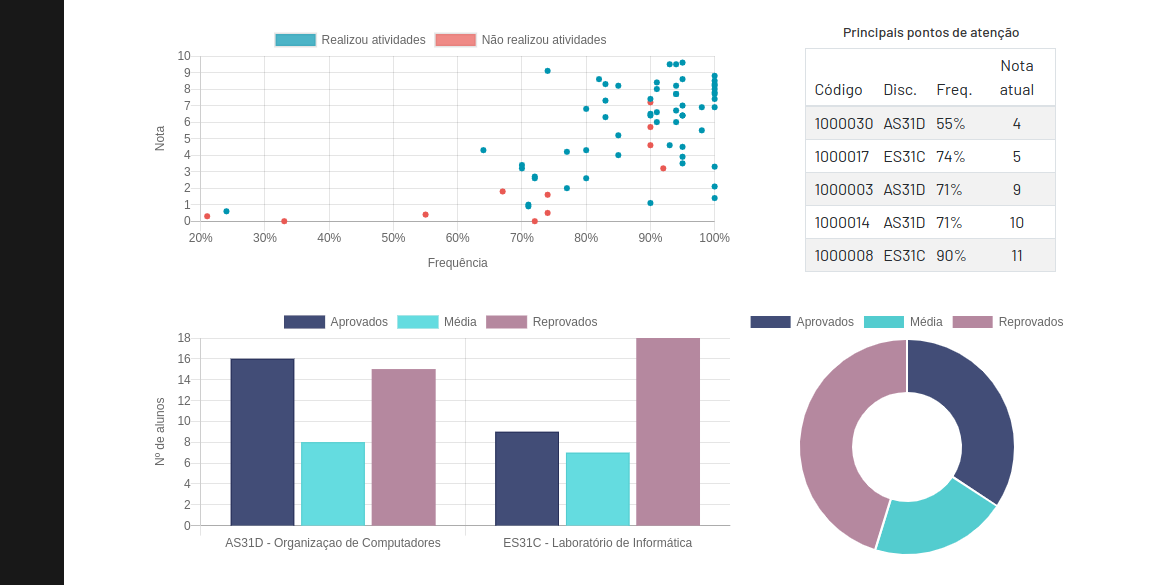
\includegraphics[width=1\textwidth]{./dados/figuras/sistema/sistema-dashboard-2}
    \fonte{Autoria Própria}
    \label{fig:dashboard-2}
\end{figure}

\subsection{Configurações}
\label{ssec:configuracoes}

Seguindo um fluxo da jornada do usuário ao utilizar a ferramenta, após a tela inicial, a próxima a ser acessada em um primeiro acesso ao sistema será a tela de configurações, esta é apresentada na figura  \ref{fig:sistema-configuracoes-1}. 

\begin{figure}[!htb]
    \centering
    \caption{Página de configurações}
    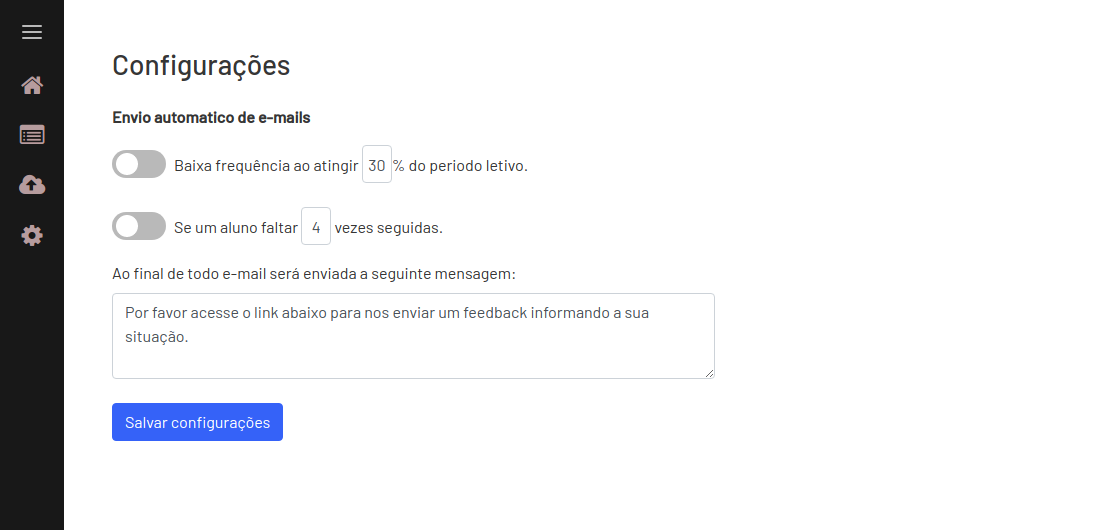
\includegraphics[width=1\textwidth]{./dados/figuras/sistema/sistema-configuracoes-1}
    \fonte{Autoria Própria}
    \label{fig:sistema-configuracoes-1}
\end{figure}

Nesta o usuário pode selecionar dois mecanismos de detecção automática no carregamento de planilhas. 
O primeiro permite que o sistema detecte ao passar uma parte do período letivo os alunos com frequência abaixo do limite de 75\%.
O segundo mecanismo permite a detecção dos alunos que faltaram múltiplas vezes em sequência, o que pode refletir em alguma situação incomum por conta do aluno, como o momento de desistência da disciplina, impedimento médico ou algum outro evento que o impossibilite de participar das aulas.

Com a detecção destes eventos o sistema permite o envio de um e-mail para todos os alunos que se enquadram nessas situações. Desta forma há um campo nesta página para que o usuário possa personalizar a mensagem a ser enviada aos alunos nestes e-mails.
O campo altera a mensagem enviada ao final de todo e-mail, ou seja, a mensagem localizada após todo o texto enviado no e-mail.

Caso habilitados, os mecanismos também dispõe um campo cada, que permite que a mensagem enviada por conta da detecção específica seja personalizada.
Como exemplificado na figura \ref{fig:sistema-configuracoes-2}, as mensagens padrões para os mecanismos são: 

\begin{itemize}
    \item Baixa frequência ao atingir \textit{30\%} do período letivo: O período letivo alcançou \#percentage do semestre e o sistema de prevenção à retenção identificou que sua frequência está abaixo do limite parcial da disciplina.
    \item Se um aluno faltar \textit{4} vezes seguidas: O sistema de prevenção à retenção identificou que você faltou \#times vezes seguidas.
\end{itemize}

\begin{figure}[!htb]
    \centering
    \caption{Página de configurações com campos expandidos}
    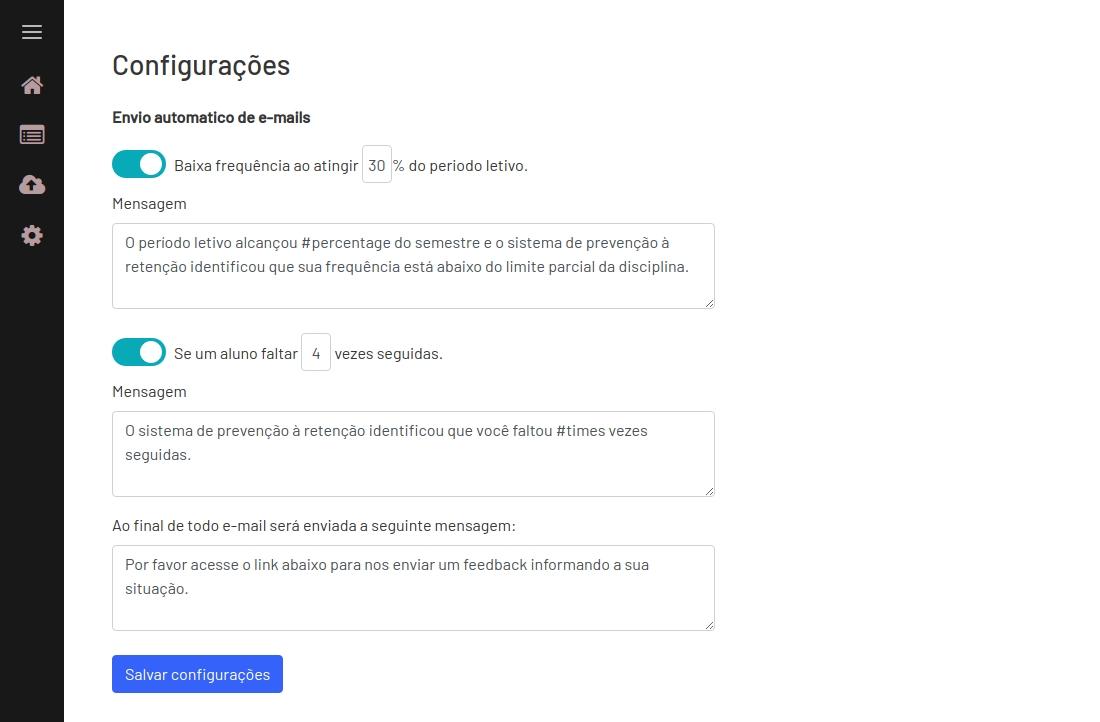
\includegraphics[width=1\textwidth]{./dados/figuras/sistema/sistema-configuracoes-2}
    \fonte{Autoria Própria}
    \label{fig:sistema-configuracoes-2}
\end{figure}

Os termos precedidos pelo símbolo \# representam variáveis que são alteradas automaticamente no envio do e-mail pelo valor gatilho selecionado para o evento. Ou seja, para este caso a expressão \#percentage será substituída por \textit{30\%} e a expressão \#times será substituído por \textit{4}.

\subsection{Upload de Dados}
\label{ssec:uploadDados}

A próxima página do fluxo de uso da ferramenta é a de upload de dados, esta é apresentada na figura \ref{fig:sistema-upload-1}. Nesta tela o usuário pode selecionar a disciplina associada aos dados que serão carregados. 

A \textit{API} em Node.js está preparada para a inserção de novas disciplinas e possui uma rota implementada para esse procedimento, porém o sistema ainda não possui uma tela de cadastro de disciplinas. 
Desta forma algumas disciplinas foram cadastradas a fim de exemplificação. 
Um dos campos esperados na inserção de uma nova disciplina no banco de dados é a data de término do período letivo, utilizado para o cálculo da frequência com base no número de aulas já dadas e faltantes.

Em seguida o usuário deve selecionar o tipo de planilha que será carregada, podendo esta ser de notas e faltas, consolidadas em um arquivo único, ou dados do URI Online Judge Academic.

Caso selecionado a opção \textit{Notas e Faltas} são exibidos campos de pesos, onde o docente deve inserir o peso das avaliações e o peso dos trabalhos para a complementação da nota final dos alunos. 
Os valores são em porcentagem, desta forma a soma dos dois pesos deve equivalente a 100. 
Ao modificar um dos campos de peso automaticamente o peso presente no outro campo será ajustado, complementando-o a 100.

Por fim seleciona-se a planilha a ser submetida e finaliza-se o envio.

\begin{figure}[!htb]
    \centering
    \caption{Página de upload de planilhas}
    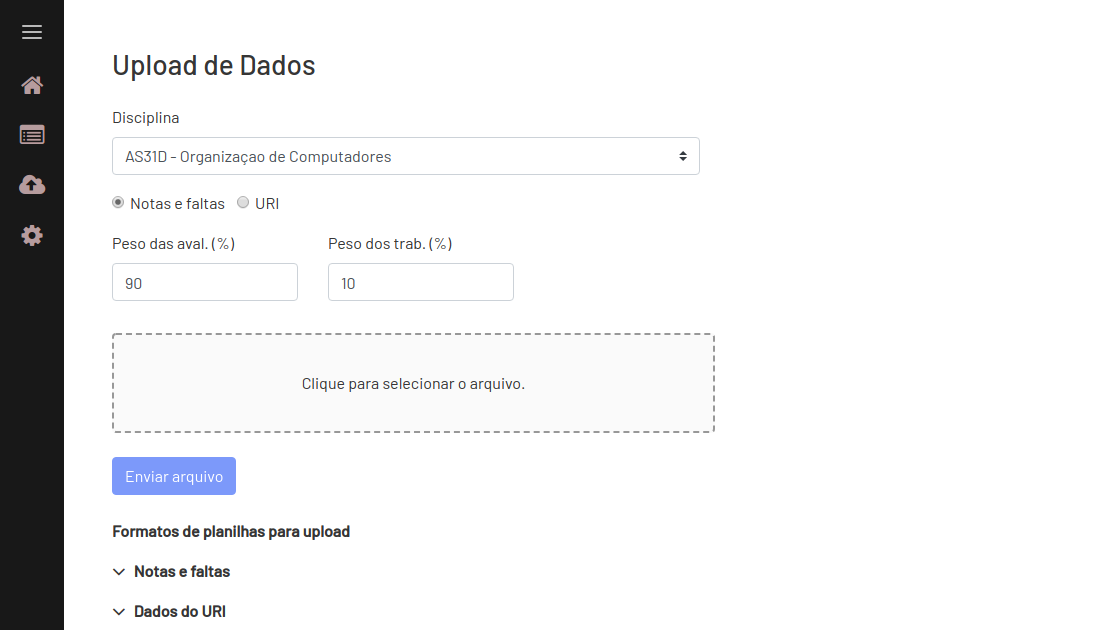
\includegraphics[width=1\textwidth]{./dados/figuras/sistema/sistema-upload-1}
    \fonte{Autoria Própria}
    \label{fig:sistema-upload-1}
\end{figure}

Na parte inferior da página é disposta uma seção guia para os usuários, com os formatos recomendados para as planilhas a serem enviadas. Ao clicar nas setas ao lado de cada opção as opções são expandidas e os \textit{layouts} são apresentados.
A figura \ref{fig:sistema-upload-2} mostra o resultado exibido na tela quando as opções estão expandidas.

\begin{figure}[!htb]
    \centering
    \caption{Página de upload de planilhas com formatos para upload expandidos}
    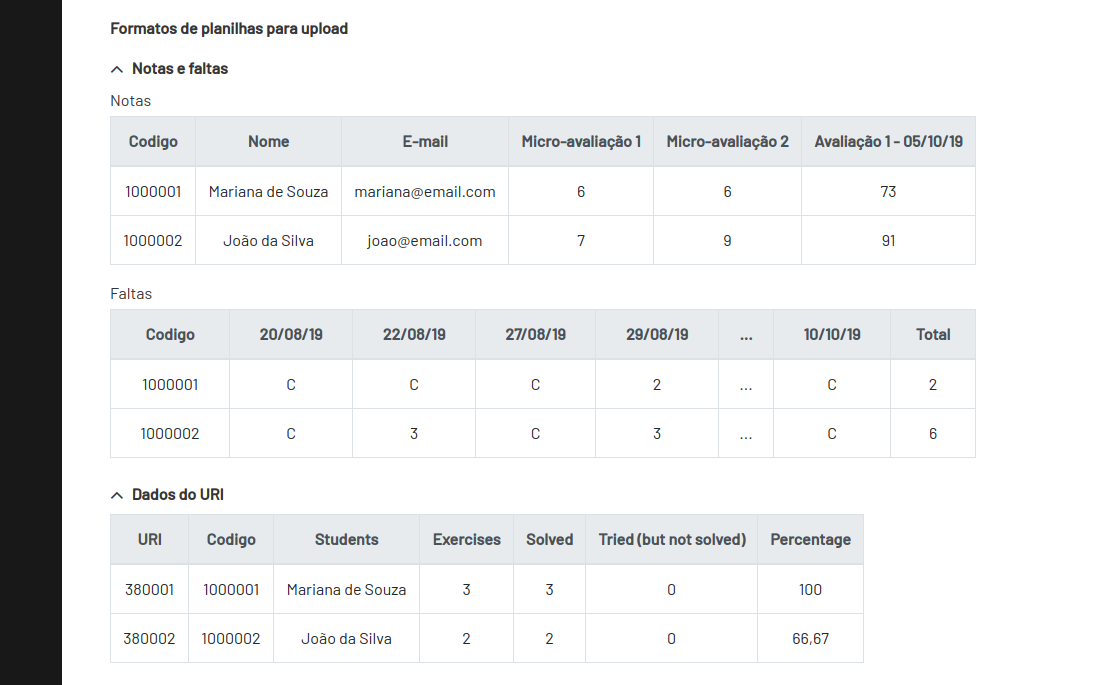
\includegraphics[width=0.8\textwidth]{./dados/figuras/sistema/sistema-upload-2}
    \fonte{Autoria Própria}
    \label{fig:sistema-upload-2}
\end{figure}

Ao finalizar o envio da planilha, internamente o sistema realizará a detecção dos alunos cujos dados se coincidem com os mecanismos assinalados na tela de configurações e exibirá uma página \textit{modal} de alerta com um resumo da situação, solicitando ao usuário a confirmação para o envio dos e-mails a todos os alunos dentro dos perfis detectados.
Caso confirmado, o e-mail é envio pelo endereço de e-mail remetente 
\textit{predicao.academica@gmail.com}, criado somente para a validação deste trabalho, e a mensagem enviada por e-mail aos alunos é construída com base nas mensagens especificadas na tela de configurações anteriormente.
A figura \ref{fig:sistema-upload-3} ilustra a situação de detecção descrita.

\begin{figure}[!htb]
    \centering
    \caption{Detecção de alunos por meio dos mecanismos de comunicação}
    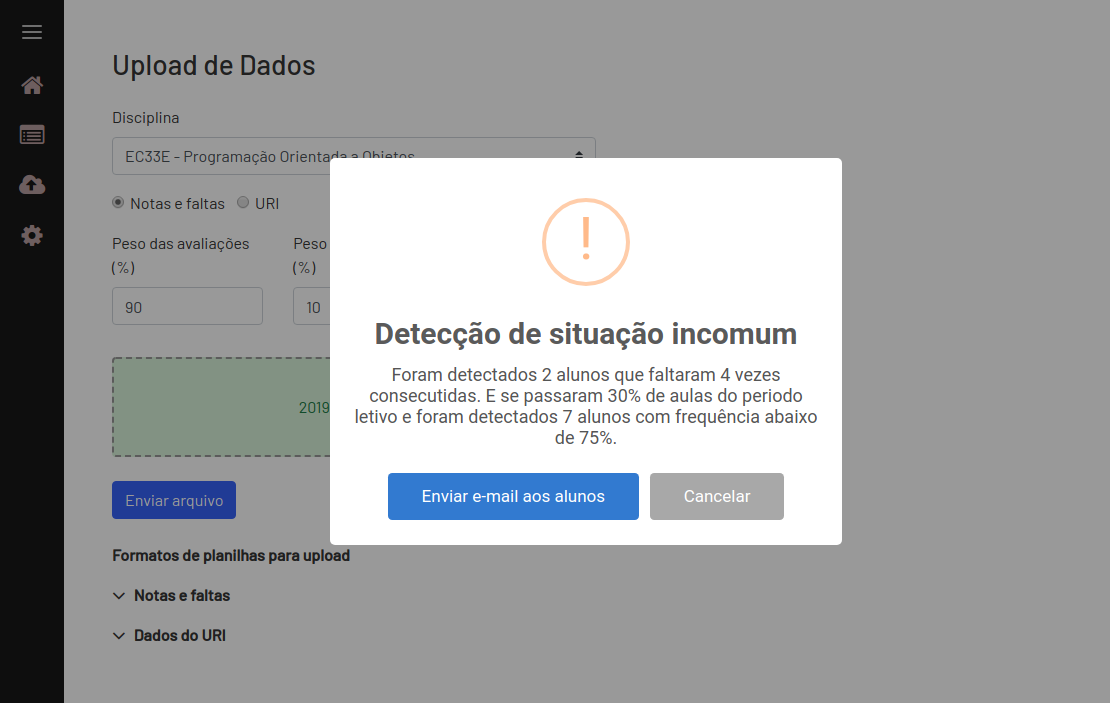
\includegraphics[width=1\textwidth]{./dados/figuras/sistema/sistema-upload-3}
    \fonte{Autoria Própria}
    \label{fig:sistema-upload-3}
\end{figure}

Para fins de validação todos os e-mails atualmente enviados pelo sistema são direcionados para \textit{lucas.franco@alunos.utfpr.edu.br}, mas a plataforma já está preparada para enviá-los para os endereços de e-mail reais dos alunos, quando estes são carregados nas planilha de notas e faltas.

\begin{figure}[!htb]
    \centering
    \caption{Exemplo de e-mail enviado à um aluno pelo sistema de predição automaticamente}
    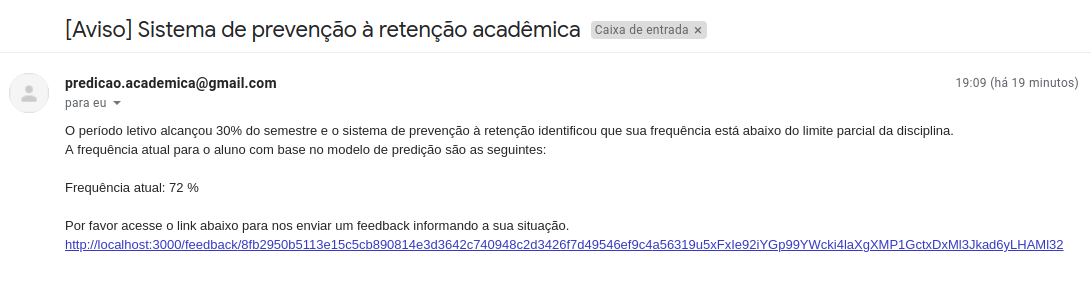
\includegraphics[width=1\textwidth]{./dados/figuras/sistema/sistema-email}
    \fonte{Autoria Própria}
    \label{fig:sistema-email}
\end{figure}

A figura \ref{fig:sistema-email} exibe um exemplo dos e-mails enviados pelo sistema automaticamente por meio da detecção.
Pode-se observar que é enviado junto à mensagem um link para que o aluno acesse. Este link é referente a próxima página a ser descrita, a página de \textit{feedback}.

\subsection{Feedback}
\label{ssec:feedback}

A página de \textit{feedback} é bastante simples e consiste de uma tela que só pode ser acessada pelo link enviado por e-mail.
Ela contém um paragrafo que explica o motivo pelo qual o e-mail lhe foi enviado e o aluno precisa enviar a justificativa, esse também é construído com base nas mensagens definidas na tela de configurações.
Além disso a tela possui um campo para que o aluno envie a justificativa. 
A figura \ref{fig:sistema-feedback} apresenta esta tela.

\begin{figure}[!htb]
    \centering
    \caption{Página de envio de feedback}
    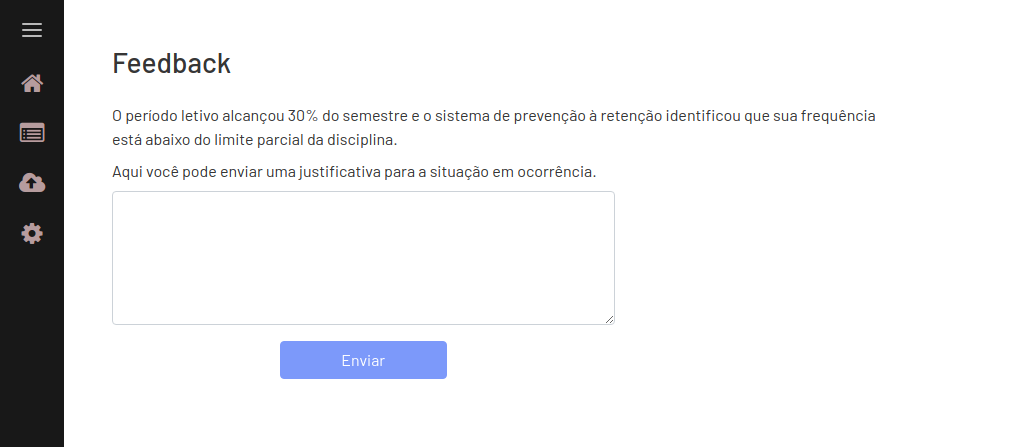
\includegraphics[width=1\textwidth]{./dados/figuras/sistema/sistema-feedback-1}
    \fonte{Autoria Própria}
    \label{fig:sistema-feedback}
\end{figure}

Na \textit{URL} gerada para o acesso a tela de \textit{feedback} são encriptados com a biblioteca \textit{SimpleCrypto} alguns dados que possibilitam identificar e armazenar o texto enviado pelo aluno. 
Entre os dados estão o código identificador do aluno, o código da disciplina e um identificador para o e-mail referente a esta justificativa, gerado ao enviar o e-mail ao aluno.

Não foi-se implementada uma tela de login nesta versão do sistema, mas ao enviar esses dados encriptados na \textit{URL} elimina-se a necessidade de um controle de acesso para os alunos, pois caso não estejam autenticados no sistema estes só poderão acessar as páginas permitidas, que neste caso é somente a tela para o envio do seu \textit{feedback}.

Ao enviar a mensagem o campo para envio da justificativa é desabilitado, assim se o estudante acessar novamente o mesmo link este não conseguirá enviar outra mensagem ou modificar a mensagem enviada.

Uma vez que o aluno envia seu \textit{feedback}, o docente poderá monitorar os e-mails enviados e as respostas recebidas na tela de detalhes do estudante.

O principal meio de acesso a tela de detalhes do estudante é por meio da página de lista. Esta é apresentada a seguir.

\subsection{Lista}

Esta página é responsável pela listagem geral dos dados dos alunos de cada turma. 
Ela é composta por uma caixa de seleção no qual o usuário escolhe a disciplina a ser listada.
A figura \ref{fig:sistema-lista-1} mostra a página de listagem para a disciplina AS31D - Organização de Computadores.

\begin{figure}[!htb]
    \centering
    \caption{Página de listagem de dados}
    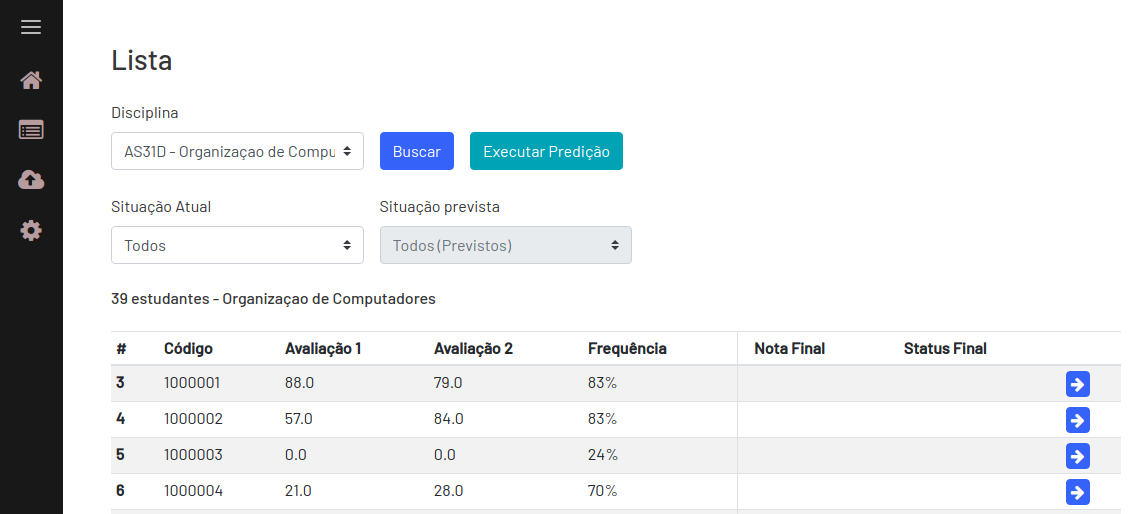
\includegraphics[width=1\textwidth]{./dados/figuras/sistema/sistema-lista-1}
    \fonte{Autoria Própria}
    \label{fig:sistema-lista-1}
\end{figure}

Em seguida estão dispostos dois botões, o primeiro é responsável por solicitar os dados armazenados no banco de dados ao \textit{back-end} em Node.js, e o segundo é responsável por realizar a chamada ao \textit{back-end} em Python, solicitando a execução dos algoritmos de \textit{machine learning} e o retorno das predições. As predições apresentadas no sistema são prevenientes do modelo criado com o algoritmo \textit{Gradient Boosting}.

A sequência de interações realizadas ao pressionar ambos os botões é ilustrada na figura \ref{fig:diagrama-2}.

Logo abaixo da caixa de seleção e botões há dois filtros, um deles é habilitado ao pressionar o botão \textit{Buscar} e permite filtrar pelas regras definidas na subseção \ref{ssec:dashboard}, e são estes: Aprovados, Média (ou limiar) e Reprovados. 
Este filtro considera a nota atual do aluno, calculado com base nas notas das avaliações e atividades.
O segundo filtro é habilitado ao pressionar o botão \textit{Executar Predição}, e permite filtrar seguindo as mesmas regras citadas anteriormente, mas considerando a nota final prevista retornada pelo modelo para os alunos.

Após a execução das predições os campos Nota Final e Status Final são preenchidos com os dados estimados pelos modelos. A figura \ref{fig:sistema-lista-2} apresenta a tela após a execução das predições.
Os alunos que obtiveram uma nota estimada acima de setenta são listados com perfil \textit{Aprovado} e os campos preenchidos são coloridos de verde. 
Para alunos que obtêm notas entre cinquenta e setenta o status apresentado é o \textit{Limiar} e os campos são coloridos de amarelo. 
Por fim os alunos com notas inferiores a 50 são sinalizados com status \textit{Reprovado} e os campos são coloridos com vermelho.

Por mais que o status \textit{Limiar} não traduza diretamente o status final do aluno, o uso desta faixa com 20\% dos pontos (entre 50 e 70) permite à ferramenta uma margem maior entre os status \textit{Aprovado} e \textit{Reprovado}, possibilitando que a determinação delicada do status do aluno com nota prevista na margem seja feita de forma mais branda. 
Porém isso requisita uma análise mais detalhada por conta do docente sobre os alunos que são designados neste perfil.

\begin{figure}[!htb]
    \centering
    \caption{Página de listagem de dados com as predições efetuadas}
    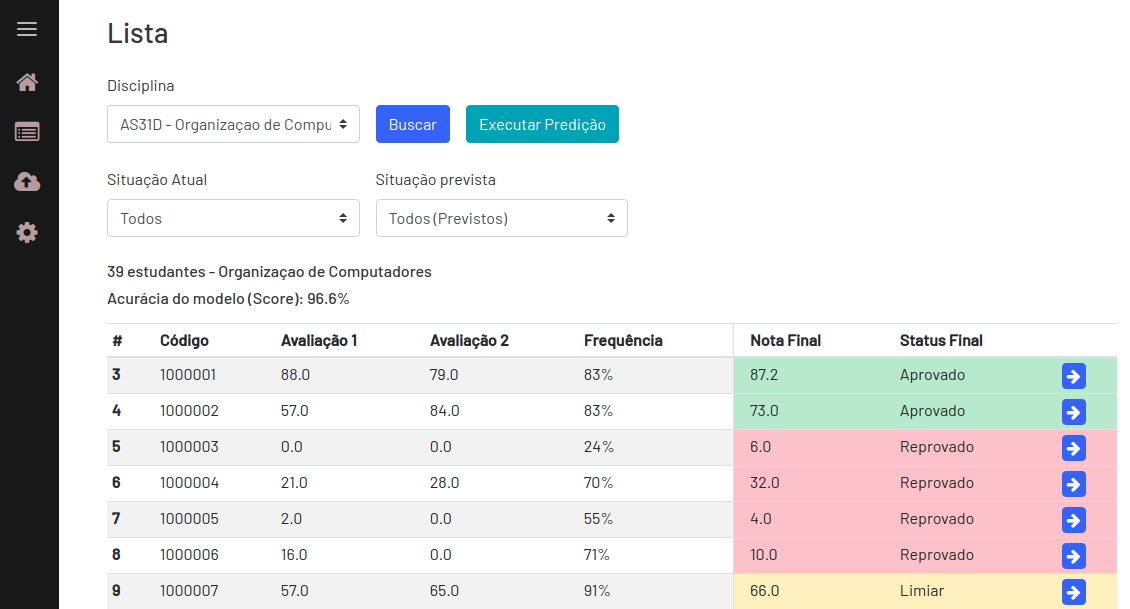
\includegraphics[width=1\textwidth]{./dados/figuras/sistema/sistema-lista-2}
    \fonte{Autoria Própria}
    \label{fig:sistema-lista-2}
\end{figure}

Ainda na tela de listagem, abaixo dos filtros é exibido o número de estudantes listados para a disciplina selecionada e a acurácia/\textit{score} do modelo utilizado para predizer as notas dos alunos.
Ao clicar em um dos botões exibidos na extrema direita de cada linha da tabela é possível acessar a tela de detalhes para o estudante selecionado.

\subsection{Detalhes do Estudante}

A página de detalhes do estudante é responsável por apresentar os dados individuais do aluno selecionado.

Como pode-se visualizar na figura \ref{fig:sistema-detalhes-1}, que ilustra a página de detalhes, esta possui um \textit{card} na parte superior da tela que apresenta o nome e R.A. do aluno, bem como a lista de disciplinas matriculadas com dados inseridos na ferramenta. 
Para cada disciplina são exibidas as notas obtidas pelo aluno até o momento, a sua frequência e a nota final prevista pelo modelo de \textit{machine learning}.

Caso a nota prevista seja igual ou superior a 70 o campo é apresentado em verde e um ícone de \textit{ok} é mostrado, caso a nota esteja entre 50 e 70 o campo é colorido de amarelo com um ícone de atenção.
E para notas inferiores a 50 o campo é apresentado em vermelho com um ícone em forma de \textit{X}.
Semelhante aos indicadores do dashboard apresentados na figura \ref{fig:dashboard-1}.

\begin{figure}[!htb]
    \centering
    \caption{Página de detalhes do estudante}
    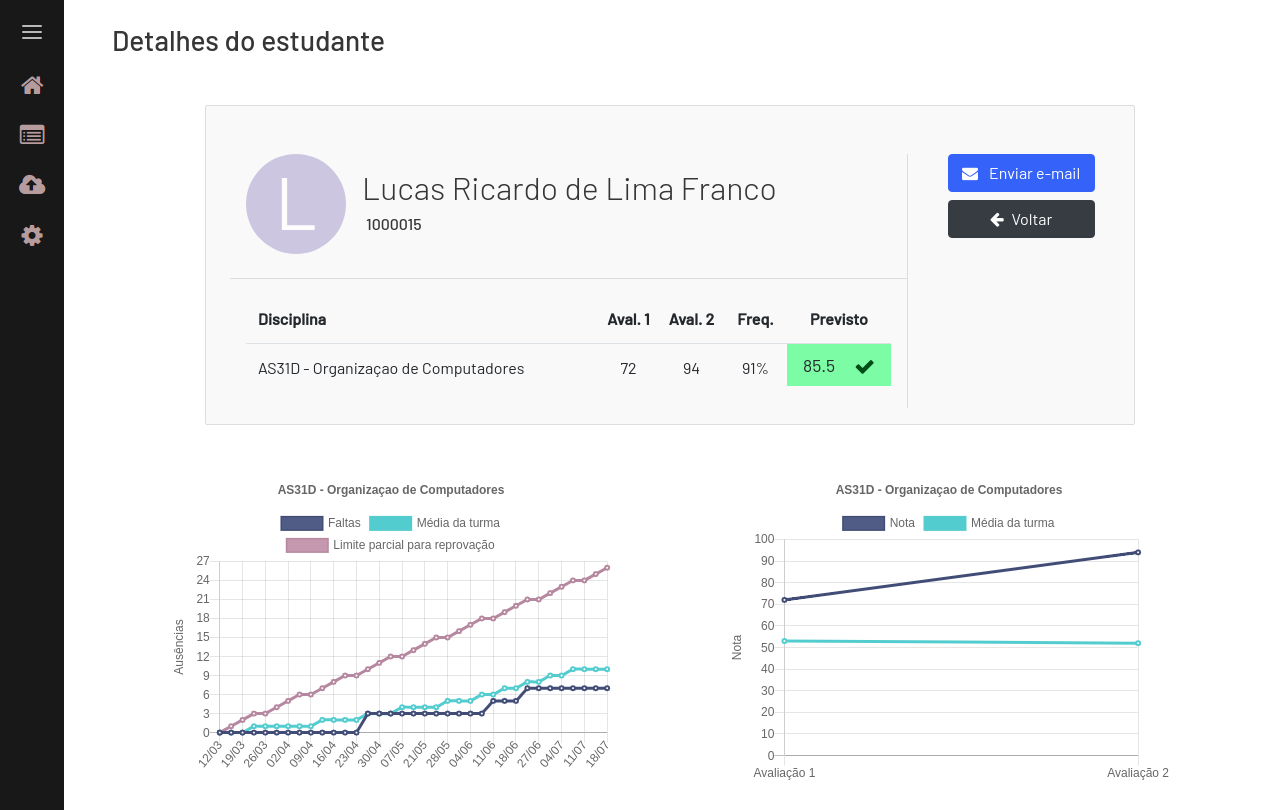
\includegraphics[width=1\textwidth]{./dados/figuras/sistema/sistema-detalhes-1}
    \fonte{Autoria Própria}
    \label{fig:sistema-detalhes-1}
\end{figure}

Abaixo do \textit{card} são gerados dinamicamente gráficos comparativos entre o desempenho do aluno e a média da turma. 
Para cada disciplina vinculada ao aluno é plotado um novo par de gráficos.
Para cada par de gráficos, o primeiro compara o número de ausências do aluno com a média da turma, trazendo também o limite de ausências que um aluno pode ter sem que ocorra a reprovação por faltas.
Já o segundo gráfico ilustra o comportamento das notas do aluno, possibilitando ver se estas estão em crescimento ou declínio, comparando-as com a média de notas da turma.

Retornando ao \textit{card} na parte superior da tela é possível verificar dois botões na sua direita. 
Um deles é utilizado para voltar a tela anterior caso desejado.
O outro é utilizado para realizar o envio de um e-mail personalizado ao aluno apresentado nesta tela, e ao clicar neste botão será apresentado uma página \textit{modal} com um campo para que o usuário insira uma mensagem a ser enviada no e-mail junto de um link gerado automaticamente para que o aluno envie um \textit{feedback}. 
A figura \ref{fig:sistema-detalhes-2} exemplifica a ação ocorrida ao pressionar o botão \textit{Enviar e-mail}.

\begin{figure}[!htb]
    \centering
    \caption{Mensagem personalizada a ser enviada no e-mail por meio da página de detalhes do estudante}
    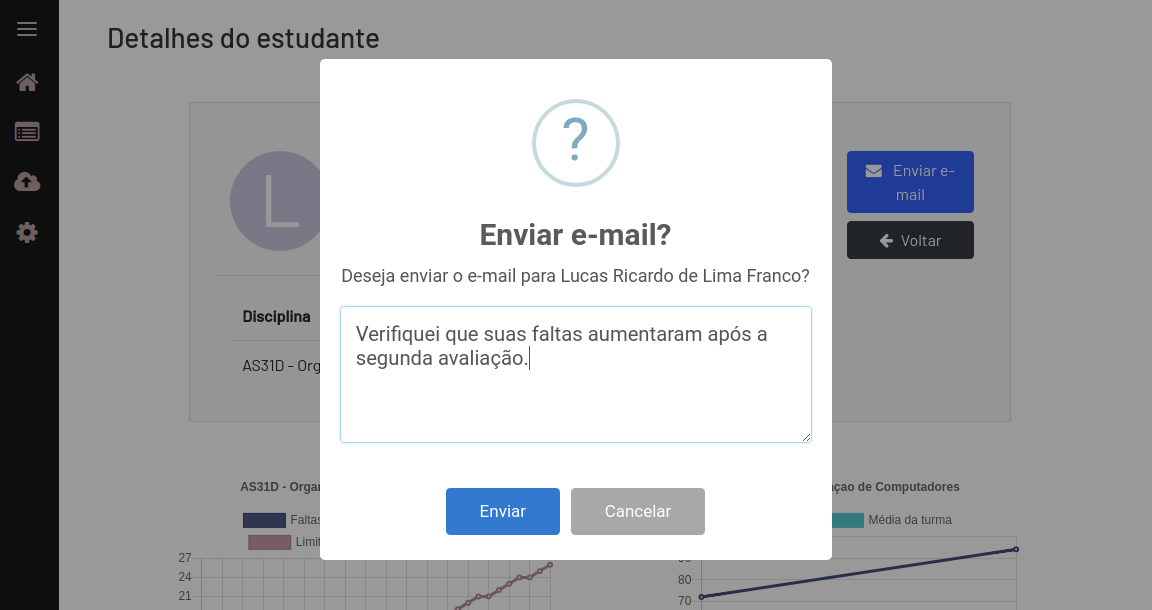
\includegraphics[width=1\textwidth]{./dados/figuras/sistema/sistema-detalhes-2}
    \fonte{Autoria Própria}
    \label{fig:sistema-detalhes-2}
\end{figure}

A figura \ref{fig:sistema-detalhes-3} apresenta o e-mail recebido pelo ação executada anteriormente, nesta é possível verificar que a construção do e-mail se deu com base na mensagem descrita na figura \ref{fig:sistema-detalhes-2}.
Ao final do e-mail se encontra o link para que o aluno acesse e envie o \textit{feedback} solicitado.

\begin{figure}[!htb]
    \centering
    \caption{E-mail enviado por meio da página de detalhes do estudante}
    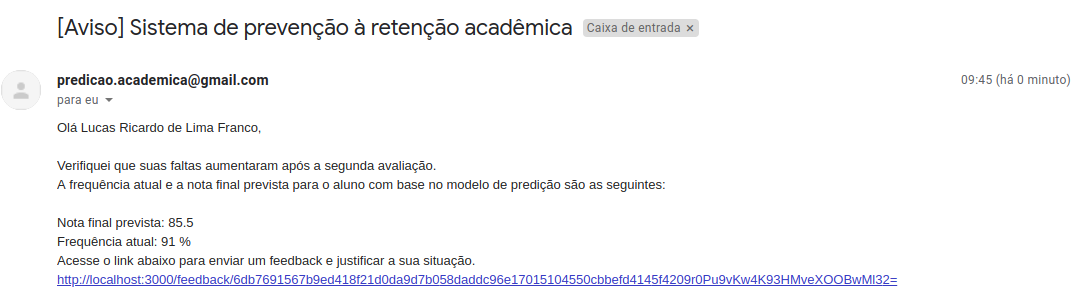
\includegraphics[width=1\textwidth]{./dados/figuras/sistema/sistema-detalhes-3}
    \fonte{Autoria Própria}
    \label{fig:sistema-detalhes-3}
\end{figure}

Por fim a tela de detalhes do estudante permite visualizar a lista de e-mails enviados ao aluno, o status destes, ou seja, se o aluno já o retornou com o seu \textit{feedback} ou se está pendente de resposta. 
Caso o aluno já o tenha respondido é possível ler a justificativa enviada.
Também são exibidas a data e hora de envio dos e-mails e da resposta do aluno, caso existente.

A figura \ref{fig:sistema-detalhes-4} exemplifica a lista de \textit{feedbacks} apresentando uma lista com dois envios de e-mail. 
Esta é ordenada por data de envio, iniciando pelos mais recentes.

O primeiro da lista é referente ao envio do e-mail da figura \ref{fig:sistema-detalhes-3}, que ainda não recebeu uma resposta do aluno.

Já o segundo é referente a uma notificação enviada ao aluno na detecção automática realizada no momento do upload das planilhas, por meio dos mecanismos estabelecidos anteriormente na tela de configurações.
Este recebeu um retorno e pode ser visto no campo \textit{Feedback} da lista.

\begin{figure}[!htb]
    \centering
    \caption{Lista de feedbacks disponível na página de detalhes do estudante}
    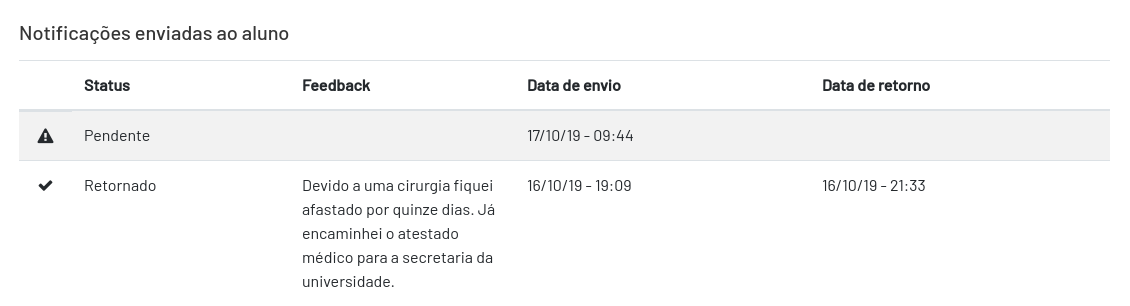
\includegraphics[width=1\textwidth]{./dados/figuras/sistema/sistema-detalhes-4}
    \fonte{Autoria Própria}
    \label{fig:sistema-detalhes-4}
\end{figure}